\documentclass[preprint]{sigplanconf-eurosys} 

%========================
%  Packages
%========================

\usepackage{graphicx,url,color}
\usepackage{amsmath}
\usepackage{amssymb}
%\usepackage{amsthm}  %<---- for a different "look" in theorems (theorem word in bold, etc.) %ACM conflict with proof definition?
%\usepackage{subfigure}
%\usepackage[tight,footnotesize]{subfigure}
\usepackage{algorithm}
\usepackage[noend]{algpseudocode}
\usepackage{times}

%\usepackage{todonotes}
%\usepackage[normalem]{ulem} %strikethrough: \sout{Hello World}
%\usepackage{lastpage} %for number of pages
%\usepackage{xspace}
%\usepackage{multirow}
%\usepackage{balance}

\usepackage[colorlinks=true,allcolors=blue,breaklinks]{hyperref}   % hyperlinks, including DOIs and URLs in bibliography
\usepackage{subcaption}
\usepackage{graphicx}
\usepackage{caption}
\usepackage{float}

%========================
%  Macros
%========================

\newcommand{\code}[1]{\textsf{\fontsize{9}{11}\selectfont #1}}

\newcommand{\inred}[1]{{\color{red}{#1}}}
\newcommand{\remove}[1]{}
\newcommand{\Idit}[1]{[[\inred{Idit: #1}]]}
\newcommand{\Yoni}[1]{[\inred{Yoni: #1}]}


\newcommand{\sys}{Lorra}
\newcommand{\sysll}{omidLL}
\newcommand{\speedup}[1]{#1$\times$}
\newcommand{\tuple}[1]{\ensuremath{\langle \mbox{#1} \rangle}}

%========================
\begin{document}

\special{papersize=8.5in,11in}
\setlength{\pdfpageheight}{\paperheight}
\setlength{\pdfpagewidth}{\paperwidth}

\conferenceinfo{CONF 'yy}{Month d--d, 20yy, City, ST, Country}
\copyrightyear{20yy}
\copyrightdata{978-1-nnnn-nnnn-n/yy/mm}
%\copyrightdoi{nnnnnnn.nnnnnnn}

% Uncomment the publication rights you want to use.
%\publicationrights{transferred}
%\publicationrights{licensed}     % this is the default
%\publicationrights{author-pays}

%\titlebanner{Draft}        % These are ignored unless
\preprintfooter{Draft - Submitted to XX}   % 'preprint' option specified.

\title{Fast Local Transactions in Distributed Data Stores}

\authorinfo{Paper ID}
           {Number of pages}
           {}

\remove{

 Aran Bergman\\
 	\affaddr{Technion -- I.I.T}\\
	\email{aranb@technion.ac.il}
\and %
Edward Bortnikov\\
	\affaddr{Yahoo Research}\\
	\email{ebortnik@yahoo-inc.com}
\and %
	Yonatan Gottesman\\
	\affaddr{Yahoo Research}\\
	\email{yonatang@yahoo-inc.com}
\and %
Eshcar Hilel\\
	\affaddr{Yahoo Research}\\
	\email{eshcar@yahoo-inc.com}
\and %
Idit Keidar\\
	\affaddr{Technion -- I.I.T}\\
	\email{idish@ee.technion.ac.il}
\and %
Ohad Shacham\\
	\affaddr{Yahoo Research}\\
 	\email{ohads@yahoo-inc.com}
 
}


\maketitle

%For ACM formats
\sloppy

%=========================================================================
%  Abstract
%=========================================================================

\begin{abstract}
TBD
\end{abstract}

%========================

\section{Introduction} \label{sec:intro}
% Transactions in big-data platforms
In recent years, transaction processing~\cite{Gray:1992:TPC:573304} technologies have paved their way into many-petabyte big data 
platforms~\cite{Percolator2010,Spanner2012,Omid2017}. 
%In some cases, they are built into the storage system itself~\cite{Spanner2012} whereas in the others they are standalone services~\cite{Omid2017}. 
Modern industrial  systems~\cite{Percolator2010,Omid2017,tephra,cockroach} complement 
existing underlying key-value storage with {\em atomicity}, {\em consistency}, {\em isolation\/} and 
{\em durability} (ACID) semantics that enable programmers to perform 
complex data manipulation without over-complicating their applications. Transaction support 
in web-scale applications started from specific use cases like real-time content indexing~\cite{Percolator2010,
Omid2017} but quickly expanded to full-scale SQL-compliant OLTP and online analytics~\cite{Phoenix, F1-2013}.

Similarly to many technologies, the adoption of transactions took a  ``functionality-first" trajectory. 
For example, the developers of Google Spanner~\cite{Spanner2012} wrote: ``We believe it
is better to have application programmers deal with performance problems due to overuse 
of transactions as bottlenecks arise, rather than always coding around the lack of transactions''. 
Yet the expectation for high performance is rapidly picking up. %For instance, 
Whereas early transaction systems were not latency-sensitive~\cite{Percolator2010, Omid2017}, 
with the thrust into new interactive domains like messaging~\cite{Borthakur:2011} and algorithmic 
trading~\cite{opentsdb}, latency becomes essential. This paper is motivated by such  applications.

Consider, for example, the platform powering Yahoo! Mail, which serves hundreds of millions of users. 
The Mail backend ingests billions of messages daily; messages undergo both machine 
classification (e.g., for spam filtering, thread detection, and ``smart views''~\cite{smart-view}),
%\footnote{\footnotesize{\url{https://yahoohelpcommunity.tumblr.com/post/118485031125/getting-to-know-smart-views-in-yahoo-mail}}}
and user manipulation (e.g., starring, tagging, and moving between folders).    
Mail users browse their mail and search for content, issuing many billions of requests a day; they
expect a consistent experience -- e.g., messages  do not 
disappear when moved between folders, starred content gets prioritized in search, folder counters are reliable, etc.

The Yahoo! Mail metadata platform is built on top of Apache HBase~\cite{hbase}, 
which provides reliable and scalable key-value storage. The system's first generation
was built without transaction support. This exposed  developers to very complex programming scenarios 
to achieve ACID behavior (e.g., consistent folder listings, atomic updates of multiple counters). 
%We would like to build the next generation of the system using a transaction API on top of HBase.
We have looked into building the next generation using  Omid~\cite{omid}, 
an Apache Incubator project which provides a transaction API on top of HBase, and 
is already in use at large scale at Yahoo~\cite{Omid2017}.
Unfortunately, while this makes programming much easier, it also jeopardizes 
the real-time latency SLA for interactive user experience. For example,  
simple updates and point queries must complete within single-digit milliseconds, 
whereas Omid, which was designed for throughput-oriented data pipelines~\cite{Omid2017}, 
can induce latencies of tens to hundreds of milliseconds under high loads. 

Motivated by this example, we have developed {\sys\/}~-- a low-latency {\em and\/} high-throughput 
transaction processing system for HBase. Similarly to other modern transaction 
managers~\cite{Percolator2010,Spanner2012,Omid2017,cockroach},
{\sys\/} provides a variant of \emph{snapshot isolation (SI)}~\cite{DBLP:conf/sigmod/BerensonBGMOO95},
which scales better than traditional serializability implementations. {\sys\/} is based on Omid~\cite{omid}, 
but dissipates the principal bottleneck present therein.
%in the prior implementations the overhead of begin and commit operations. 
Its advantage is maximized for short  transactions, which are prevalent in latency-sensitive applications.
\sys\ processes  such transactions in a handful of milliseconds. The new protocol  also doubles the system 
throughput.
%Moreover, it is amenable to a simpler high availability solution than the original design. 
%, which is \inred{an order of magnitude higher than} previously achievable limits. 
%Different aspects of our protocol are inspired by other systems, while their combination is novel.
%, to the best of our knowledge. 

As a separate contribution, we introduce a novel {\em fast path\/} algorithm for short single-key transactions 
that eliminates the begin/commit overhead entirely, and executes short transactions 
 almost as fast as native HBase operations. This entails minor extensions to the underlying 
data store. The fast path is orthogonal to other protocol aspects, and can be  supported in other 
transaction processing services. 
%, to enable local commits directly within the storage layer and verify the correctness of general 
%transactions in presence of such commits. 

We have implemented {\sys\/}\footnote{\url{https://github.com/yonigottesman/incubator-omid/tree/localTransactions}} 
based on the open source Omid code\footnote{\url{https://omid.incubator.apache.org}}, 
and extended the HBase code to enable fast path transactions\footnote{\url{https://github.com/yonigottesman/hbase_local_transactions/tree/0.98-add-rmw}}. 
Our experiments on mid-rage hardware show substantial performance improvements.
Under low load,
even without the fast path, \sys\ transactions are 4x to 5x faster than Omid's, 
and the fast path further reduces the latency of short transactions by 1.8x on average.
As system load increases, Omid's latency surges (at  $\sim\!\!\!150$K tps in our tests),  
whereas \sys's remains stable until we generate a higher load ($\sim\!\!\!250$K tps), and 
increases four-fold at 500K tps.  Fast path transactions incur no scalability
bottlenecks, and continue to execute at the low latency of native HBase operations regardless of system load,  
(thanks to HBase's near perfect scalability).
This comes at the cost of a minor (less than 15\%) negative impact on longer transactions. 
%{\inred{The system scales beyond 1M transactions per second on medium-end hardware,
%which surpasses Omid at least 4x.}} 
Additionally, \sys\ has negligible impact on  transaction abort rates.

% \Idit{The roadmap below is not essential; maybe replace with summary of contributions.}
The remainder of this paper is organized as follows:
In Section~\ref{sec:api} we define the  API and semantics of a transaction processing service. 
Section~\ref{sec:ll} presents \sys, without the fast path, and 
%Section~\ref{sec:ha} discusses its high availability mechanism. 
Section~\ref{sec:alg} then describes our support for fast path  transactions.  
Section~\ref{sec:eval} presents an empirical evaluation.
%In Section~\ref{sec:context} we generalize the fast path algorithm, and explain how it could be implemented in other systems. 
We review related work in Section ~\ref{sec:related} and conclude with Section~\ref{sec:conclusions}.


\Idit{The roadmap below is not essential; maybe replace with summary of contributions.}
The remainder of this paper is organized as follows:
We begin by providing the context for this work:   in Section~\ref{sec:api} we define the  API and semantics of a TPS, 
and    Section~\ref{sec:context} surveys  the design space of popular TPS implementations, 
highlighting the common properties of TPSs that can benefit from our approach. 
In Section~\ref{sec:new-api} we propose our extended TPS API, which provides a fast-path for local transactions. 
Section~\ref{sec:alg} then describes our algorithm for supporting fast-path local transactions.  
Section~\ref{sec:lorra} presents \sys, our low latency transaction processing system, where our fast-pass service is implemented, 
and Section~\ref{sec:eval} presents its evaluation. 
We review related work in Section ~\ref{sec:related} and conclude with Section ~\ref{sec:conclusions}.

\section{Transaction API and Semantics} \label{sec:api}


\sys\ is a \emph{Transaction Processing System (TPS)}, namely a service that runs atop an underlying data store and 
allows users to bundle multiple data store operations into a single atomic transaction. 
The TPS architecture is depicted in Figure~\ref{fig:components}.
We describe the data model and API of the underlying data store in Section~\ref{ssec:data-model}, and 
then proceed to define  the transaction semantics provided by \sys\ in Section~\ref{ssec:transactions}. 

\begin{figure}
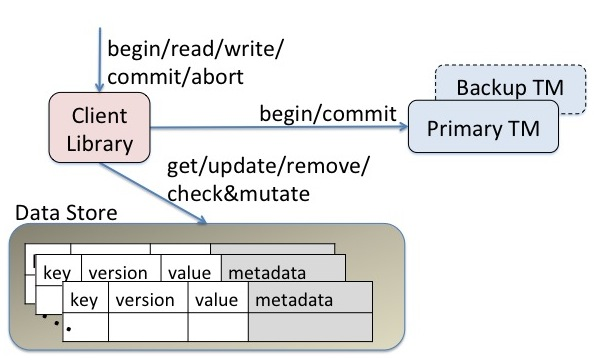
\includegraphics[width=0.48\textwidth]{FragolaComponents.jpg}
\caption{Transaction processing architecture: A client library exposes an  API for  executing transactions of data store operations. 
A centralized Transaction Manager handles transaction begin and commit requests, while data is written directly to the underlying data store.
The TM has a backup for high availability.}
\label{fig:components}
\end{figure}

\subsection{Data store}
\label{ssec:data-model}

The  data store holds  \emph{objects} (often referred to as \emph{rows}) identified by unique \emph{keys}.
Each row can consist of multiple \emph{fields}, representing different \emph{columns}. 
We consider multi-versioned objects, where object values are associated with \emph{version numbers}, and
multiple versions associated with the same key may co-exist in the data store.
\remove{
Thus, at any given time, an object holds a tuple \tuple{key,\tuple{version,value}+}, where value
can be structured to consist of multiple columns.
}
We further assume that a write operation can specify the version number it writes to.
%monotonically increasing ??
%\paragraph{API} 
The  data store provides the following API:
\begin{description}
\item [\code{get(key, version)}] --  Returns the requested version of the requested key.
%if no version is provided, returns the latest; 
%if no field is provided returns the entire record. 
%\item 
The API further allows traversing (reading) earlier versions of the same key in descending order.
\item [\code{update}(key, version, fields, values)] -- 
creates or updates an object, setting the specified fields to the specified values. 
If the version already exists, its value is updated; otherwise, a new version is added. 
\remove{The data store may buffer the write in memory until an ensuing flush. }
\item [\code{remove(key, version)}] -- removes an object with the given key and version.
\item [\code{check\&mutate}(key, version, field, old, new)] -- checks the record associated with key and version. 
If field holds old, replace it with new   and return true; otherwise return false.
\remove{ \item [\code{flush}] -- persists all previous updates to disk.}
%data stores often provide means to atomically read and update a single object, e.g., HBase exports check\&mutate operations, which are 
%internally implemented using a per-row RW lock.
%, whereas BigTable supports row transactions. 
%We will extend this capability below in order to implement certain atomic operations at the data store level.
\end{description}

A separate process performs garbage collection of obsolete versions.

\subsection{Transaction semantics} \label{ssec:transactions}

TPSs provide \emph{begin} and \emph{commit} APIs for delineating transactions: 
a \emph{transaction} the sequence of \emph{read} and \emph{write} operations on different objects 
that occur between begin and commit. Note that transactional reads and writes are implemented using the 
datastore's get and put operations.
Two transactions are said to be \emph{concurrent} if 
their executions overlap, i.e., one of them begins between the begin time and commit time of the other;
otherwise, we say that they are \emph{non-overlapping}.

A TPS  ensures the ACID properties for transactions:
\emph{atomicity} (all-or-nothing), \emph{consistency} (preserving each object's semantics), 
\emph{isolation} (in that concurrent transactions do not see each other's partial updates), and 
\emph{durability} (whereby updates survive crashes).

Different isolation levels can be considered for the third property. We consider a variant of 
snapshot isolation~\cite{DBLP:conf/sigmod/BerensonBGMOO95} that, similarly to \emph{generalized snapshot isolation}~\cite{DBLP:conf/srds/ElniketyZP05}, relaxes  the real-time order requirement. 
Nevertheless, our implementation only relaxes the ordering of fast path  transactions (described in Section~\ref{sec:alg}) 
relative to regular ones (that do not use the fast path); regular transactions continue to satisfy SI amongst themselves. 

Our correctness condition satisfies the key ``snapshot'' property of SI, which ensures that a transaction reading from the  database
does not see a mix old and new values. For example, if a task updates the values of two stocks, 
then no other transaction may observe the old value of one of these stocks and the new value of the other.
However, it relaxes the real-time order guarantee of SI by allowing (fast-path) transactions to take effect `in the past'.  
 \remove{ 
Similarly, a regular transaction overlapping
two fast path ones may observe an update of the second and miss an update by the first,  as illustrated in 
}
Figure~\ref{fig:ltx-rt}, shows an example where fast path transaction FP2 is ordered `in the past'.
%Yet we do enforce real-time order on regular transactions as well as on all updates of the same key.

\begin{figure}[ht]
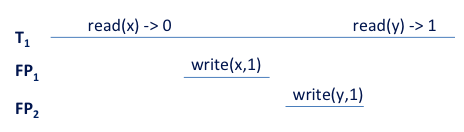
\includegraphics[width=\columnwidth]{figs/FP-semantics}
\caption{Possible violation of real-time order among fast path transactions. Regular transaction $T_1$
reads $x$ before it is updated by fast path transaction $FP_1$ and reads $y$ after it is updated by fast path transaction $FP_2$ even 
though $FP_2$ occurs after $FP_1$. 
%$T1$'s global version is $10$, and its skips the local version clocks of the regions holding $x$ and $y$ to $10$ when reading from them.
}
\label{fig:ltx-rt}
\end{figure}

Specifically, our correctness condition stipulates that
the system enforces a total order ${\cal T}$ on all committed transactions, so that
\begin{enumerate}
    \setlength{\itemsep}{0pt}
    \setlength{\parskip}{0pt}
    \setlength{\parsep}{2pt}  
%\item
%regular transactions (though not FP ones) are ordered in ${\cal T}$  according to their commit times;
\item
non-overlapping transactions 
%(regular and FP) 
that update the same key occur in ${\cal T}$  in order of their commit times;
\item
each  transaction's read operations see a consistent snapshot of the database reflecting 
a prefix of  ${\cal T}$; 
%and  
%that includes at least all regular transactions committed prior to its start time; and 
\item
 a transaction commits only if none of the items it updates is modified by a transaction ordered in ${\cal T}$ after
 its snapshot time and before its commit time.
 \end{enumerate}

\remove{ % OLD SI definition - no relaxation of RTO
More precisely, 
SI enforces a total order on committed transactions according to their commit times so that 
\begin{enumerate}
    \setlength{\itemsep}{0pt}
    \setlength{\parskip}{0pt}
    \setlength{\parsep}{2pt}  
\item
each transaction's read operations see a consistent snapshot of the database reflecting write operations by
 exactly those transactions that committed prior to the transaction's start time; and 
\item
 a transaction commits only if none of the items it updates has been modified since that snapshot.
 \end{enumerate}
 } %Remove
 
Note that as with SI, two concurrent transactions conflict only if they both \emph{update} the same item.  
In contrast, under serializability, a transaction that updates an item also conflicts with transactions that \emph{read} that item. 
Snapshot isolation is thus amenable to implementations (using multi-versioning) that 
allow more concurrency than serializable ones, and hence scale better.
It is therefore provided by popular database technologies such as Oracle, PostgreSQL, and SQL Server,
and TPSs such as Percolator, Omid, Tephra, and  CockroachDB.

Following a commit call, the transaction may successfully \emph{commit}, whereby all of its operations take effect;
in case of conflicts, (i.e., when two concurrent transactions attempt to update the same item), the transaction may
\emph{abort}, in which case none of its changes take effect. 



%An abort may also be initiated by the programmer, e.g., 
%on encountering an error. Applications typically retry a transaction upon  abort. 


%%%The data is \emph{partitioned} (or sharded), and each object belongs to one region. 
%%%%Global transactions may span multiple regions, and atomically commit or abort on all. 
%%%\emph{Local transactions} are ones that access a single region.


\section{Context and Applicability} \label{sec:context}

This section outlines the general characteristics of transaction processing systems that can benefit from our 
suggested ``fast-path'' for handling short local transactions. 
We consider a TPS  that spans multiple regions (sometimes called nodes, domains, or shards) and supports global
(multi-region) transactions. Data is stored in an underlying NOSQL key-value store, 
such as HBase~\cite{hbase}, BigTable~\cite{bigtable-osdi06},  or
RocksDB~\cite{rocksdb}. Clients access the data store directly, and partake in transaction
coordination, possibly using the assistance of a TM.

We first describe the data model and API of the underlying data store (Sections~\ref{ssec:data-model}).
%and~\ref{ssec:api}, respectively). 
We then proceed to define  the transaction semantics provided by the TPS
(Section~\ref{ssec:transactions}). Finally, we overview a generic schema for managing global transactions 
(and conflict resultion), which is used in the TPSs we target (Section~\ref{ssec:global-transactions}).
TPSs that adhere to this schema include Percolator~\cite{Percolator2010}, Omid~\cite{OmidICDE2014}, Tephra~\cite{tephra}, and CockroachDB~\cite{cockroach}.
%\idit{Need to check about the cockroach.}

\subsection{Data store}
\label{ssec:data-model}

The underlying data store holds  \emph{objects}  identified by unique \emph{keys}; with HBase and BigTable this refers to rows.
We consider multi-versioned obejcts, where object values are associated with \emph{version numbers}, and
multiple versions associated with the same key may co-exist in the data store.
Thus, at any given time, an object holds a tuple \tuple{key,\tuple{version,value}+}, where value
can be structured to consist of multiple columns.
We further assume that a write operation can specify the version number it writes to.
%monotonically increasing ??

The data is \emph{partitioned} (or sharded). Each object belongs to one region
(node, partition, shard, domain). \emph{Local transactions} are ones that access
a single region.

\paragraph{API} 

The underlying data store provides the following API:
\begin{description}
\item [\code{\tuple{version,value} read(key)}] -- atomically returns the value with
the highest version associated with key along with its version.
\item The API further allows traversing (reading) earlier versions of the same
key in descending order.
\item [\code{write(key,value,version)}] -- atomically creates or updates the version:
\remove{If the provided version number is smaller than the key's latest stored version, the update fails.} 
if the version already exists, its value is updated;
otherwise, a new version is added. Garbage collection of obsolete versions is a separate
process.
\item [Read-modify-write] --  data stores often provide means to atomically read and
update an object, (e.g., HBase exports CheckAndMutate operations, which are 
internally implemented using a RW lock, whereas BigTable supports row transactions). We
will extend this capability below in order to implement certain atomic
operations at the data store level.
\end{description}

\subsection{Transaction semantics} \label{ssec:transactions}

A \emph{transaction} is a sequence of read and write operations on different objects that ensures the so-called ACID properties:
\emph{atomicity} (all-or-nothing execution), \emph{consistency} (preserving each object's semantics), 
\emph{isolation} (in that concurrent transactions do not see each other's partial updates), and 
\emph{durability} (whereby updates survive crashes).

Different isolation levels can be considered for the third property. We consider systems providing  
snapshot isolation~\cite{DBLP:conf/sigmod/BerensonBGMOO95}, 
which is provided by popular database technologies such as Oracle, PostgreSQL, and SQL Server.

Intuitively, SI ensures that the information a transaction retrieves from the database 
does not mix old and new values. For example, if a task updates the values of two stocks, then no other transaction may observe the old value of one of these stocks and the new value of the other. 
%
More precisely, SI enforces a total order on committed transactions according to their commit times so that 
\begin{enumerate}
    \setlength{\itemsep}{0pt}
    \setlength{\parskip}{0pt}
    \setlength{\parsep}{2pt}  
\item
each transaction's read operations see a consistent snapshot of the database reflecting write operations by
 exactly those transactions that committed prior to the transaction's start time; and 
\item
 a transaction commits only if none of the items it updates has been modified since that snapshot.
 \end{enumerate}
Thus, under SI, two concurrent transactions conflict only if they both \emph{update} the same item.  
In contrast, under serializability, a transaction that updates an item also conflicts with transactions that \emph{read} that item. Snapshot isolation is thus amenable to implementations (using multi-versioned concurrency control) that 
allow more concurrency than serializable ones, and hence scale better.

TPSs allow programmers to  delineate transactions via the begin and commit APIs: 
the sequence of read and write operations a client invokes between begin and  commit pertains to one transaction.
Following a commit call, the transaction may successfully \emph{commit}, whereby all of its operations take effect;
in case of conflicts, (i.e., when two concurrent transactions attempt to update the same item), the transaction may
\emph{abort}, in which case none of its changes take effect. An abort may also be initiated by the programmer, e.g., 
on encountering an error. Applications typically retry a transaction upon (either type of) abort. 
Global transactions may span multiple regions, and atomically commit or abort on all. 

\subsection{Global transaction flow} \label{ssec:global-transactions}

A TPS's API is offered by a client library, which accesses the data directly in the data store, and 
performs coordination actions to begin, commit, or abort transactions. 

The TPSs we consider all rely on versions for coordination: when a transaction begins it obtains a \emph{tentative version}, which 
it uses (1) to determine what version of each key to read; and (2) as the version of data items it writes.   
In Percolator, Omid, and Tephra, as well as our implementation in this paper, timestamps are provided by a monotonically
increasing \emph{global version  clock (GVC)}. CockroachDB instead provides the beginning transaction with the local clock of
one of the regions (called node therein), which is closely synchronized relative to other regions and furthermore ensures causality.

Transactions indicate their intention to write to an object; this is done using
a dedicated column (part of the value in our data model), which keeps logical
(application-level) locks in some implementations (Percolator) and tentative
updates in others (e.g., the new version of Omid~\cite{Omid-blog}, and CockroachDB). 
While write intentions differ across implementations, we assume that the following generic boolean function is  provided:
\begin{description}
\item[\code{hasWriteIntent(key, version)}] returns true if the specified version of key has a write intent indication; if version is not provided, the 
latest version associated with key is checked.
\end{description}

Note: in certain implementations (like the virtual lock per-key used in Percolator), the write-intent of all versions associated 
with the same key is the same, whereas in other cases (like Omid, which uses tentative versions), a
new version may have a write intent while an older one does not.

A transaction goes through the following phases:
\begin{enumerate}
  \item{Begin} -- A transaction obtains a tentative version number when it starts. 
  It also obtains a unique transaction id.
  The two can be combined (i.e., the tentative version can be the same as the  transaction id).
  \item{Collect reads and indicate write intention} -- (either jointly or  collect first and then write).
  	\begin{itemize}
  		\item  \emph{Collect} means reading object values  and versions; each object atomically. 
  		Only versions committed with timestamps  smaller or equal to the transaction's tentative version are read. 
  		Encountered write indications by uncommitted transactions are dealt with differently in different systems, e.g., Percolator 
  		waits for the indication to be lifted, Omid ignores uncommitted versions and checks for conflicts this may induce at
  		commit time, and CockroachDB forces the transaction with the write indication to either commit with a higher version 
  		than its own tentative version, or abort. Similarly, the solution we implement in this paper forces the transaction with the write 
  		indication to abort. 
  		Collect occurs during the transaction (encounter time).
  		\item \emph{Indicating write intention} changes the objects' write intention columns
  		to indicate a transaction attempting to write them is under way. The value the
  		transaction intends to write is added with a new version. In Omid, this
  		version is the transaction's id. Each object is updated atomically. This can
  		occur either at encounter time or at commit time, in which case it occurs as the first phase of the commit. 
  	\end{itemize}
  \item{Validation/conflict detection} -- Before a transaction can commit, it must check that it does not conflict with any 
  concurrent transactions.  For SI, we need to check for write-write conflicts only. 
  This step checks write intentions as well as version numbers. It is performed differently in different systems.
  \item{Commit} --  In case validation succeeds, the transaction may be committed 
  in one atomic step to a designated \emph{commit entry}, which can reside in a global table (like the Commit Table of 
  the new version of Omid and the Transaction Table of CockroachDB) or alongside the first  key written by 
  the transaction (as in Percolator and the implementation in this paper).  Note that a commit attempt may
  fail and abort instead. 
  \item{Clean-up} -- changes the write intentions of the transaction to
  persistent writes in case of commit, and removes them in case of abort. This
  phase occurs after the transaction is persistently committed or aborted, in
  order to reduce the overhead of future transactions and garbage collect
  obsolete information. 
  \remove{Note that whenever a transaction encounters a write
  indication in the collect phase it must access the commit entry in order to
  check the transaction's commit status. Once the clean-up phase is over, future
  transactions no longer incur this overhead for keys updated by the terminated
  transaction.}
\end{enumerate}

 

\section{Introducing Fast Path Local Transactions} \label{sec:new-api}


The goal of our fast path  is to forgo the overhead associated with two-phase transaction processing and communication with 
the (possibly remote) TM. This is particularly important for short transactions, where the begin and commit overhead is not amortized
across many operations.
\inred{Can we give some example workload?}

To this end, we introduce in Section~\ref{ssec:fast-api} a streamlined API that jointly executes multiple API calls of the original TPS;
we refer to transactions that use this API as \emph{fast path (FP) transactions}. We 
then discuss the semantics of FP transactions relative to regular ones.
% in Section~\ref{ssec:fast-semantics}.

\inred{Explain regions!}

We proceed to explain our support for local transactions with SI semantics in the
context of a system following the generic schema of  Algorithm~\ref{alg:schema} above. 
Our solution consists of three parts: First, in Section~\ref{ssec:region-clock}, we enhance the
underlying data store with support for per-region \emph{Local Version Clocks (LVCs)}. 
This aspect is already implemented in CockroachDB, which uses 
per-region Hybrid Logical Clocks~\cite{Kulkarni2014LogicalPC} in order to allow for distributed timestamp allocation. 
In the systems that maintain a GVC, (e.g.,~\cite{Percolator2010,tephra,OmidICDE2014,omid-blog}), our 
addition of  LVCs 
entails a minor modification to management of global timestamps (in the transaction manager or oracle). 
Second, in Section~\ref{ssec:lvc-access}
we extend the underlying data store's API to allow manipulating 
a region's LVC jointly with objects stored at that region. 
Finally, we add client-side support for the fast path API, as explained in Section~\ref{ssec:lc-client}.


\subsection{API and semantics}
\label{ssec:fast-api}

\paragraph{API.}
For brevity, we refer to the TPS's API calls  begin, read, write, and commit as \code{b, r, w}, and \code{c} respectively, and 
we combine them to allow fast processing.
The basic FP transactions are singletons, i.e., transactions that perform a single
read or write. These are supported by the APIs: 
\begin{description}
\item[brc(key)] -- begins an FP transaction, reads key within it, and commits.
%Recall that read-only transactions don't need to commit. 
\item[bwc(key,val)] -- begins an FP transaction,  writes val into a new version of key that exceeds all existing ones, and commits.
\end{description}

We further support a fast path transaction consisting of a read and a dependant write, via a pair of API calls:
\begin{description}
\item[br(key)] -- begins an FP transaction and  reads the latest version of key.
\item[wc(key,val)] -- 	validates that key has not been written since the last \code{br} call, writes val into a new version of key, and commits.
\end{description}

\remove{
A more elaborate example is a read-modify-write API: 
\begin{description}
\item[brwc(key,f)] -- begins an FP transaction,  reads the latest version of key, applies $f$ to it (on the server side), 
	writes the result into a new version of key that exceeds all existing ones, and commits.
\end{description}

To use the above API, the programmer has to encapsulate the transaction logic in a function for server-side processing. 
Alternatively, we allow FP transactions to unfold dynamically much like regular  transactions do.
A dynamic FP transaction may instead begin with a \code{br} call, perform client-side processing, and then call the following
function to update either the same or a different key: 

\begin{description}
\item[wc(key,val)] -- writes val into a new version of key that exceeds all existing ones, and commits.
\end{description}

Moreover, we do not restrict FP transactions to perform a single read -- any number of \code{r}'s may be called between the \code{br} 
and \code{wc}. The supported types of FP transactions are summarized in Table~\ref{table:fp-types}.
Note, however, that all calls must be directed at the same region, else the transaction is not local.
In case an FP transaction dynamically discovers that it needs to access additional regions, it is aborted and should be restarted as a regular transaction. 

\begin{table}[htb]
%\def\arraystretch{1.5}%  1 is the default, change whatever you need
\centerline{
\begin{tabular}{l  @{\hspace{2em}} l}
Call sequence & Transaction type\\
\hline
\code{br} & single read\\
\code{bwc} & single write\\
\code{br, r*} &  multi-read\\
\code{br, r*, wc} & multi-read, single write\\
\code{brwc} & server-side single-read-write\\
%\hline
\end{tabular}
}
\caption{Supported FP transaction types.}
\label{table:fp-types}
\end{table}

In principle, it would have been possible to also allow \code{w} calls in the span of an FP transaction, 
but in this case, it is not possible to forgo the two-phase execution. 
That is, the \code{w} calls would need to indicate write intents, and  to be atomically committed (or aborted) during the final \code{wc} 
(or \code{c}) call. 
Given the limited benefit and extra complexity of allowing many writes in FP transactions, we do not support this option in our solution.

}

\paragraph{Semantics.}
%\label{ssec:fast-semantics}

The semantics for ordering FP transactions relative to regular ones are
weaker than SI in that they do not guarantee real-time order over all regular
and FP transactions together. Specifically, a regular transaction overlapping
two FP ones that access different regions may observe an update of
the second and miss an update by the first. For example, assume objects $x$ and $y$
are managed in two different regions, then real-time order can be violated as
illustrated in Figure~\ref{fig:ltx-rt} (ignore the skip operations for now; they will be explained in the next section).

\begin{figure}[h]
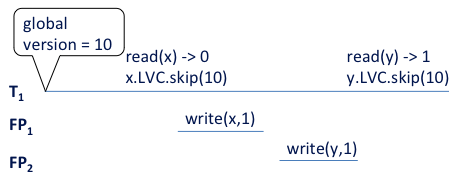
\includegraphics[width=\columnwidth]{figs/LTX-RT}
\caption{Possible violation of real-time order among fast path (FP) transactions in different regions. Global transaction $T_1$
reads $x$ before it is updated by FP transaction $FP_1$ and reads $y$ after it is updated by FP transaction $FP_2$ even 
though $FP_2$ occurs after $FP_1$. $T1$'s global version is $10$, and its skips the local version clocks of the regions holding $x$ and $y$ to $10$ when reading from them.}
\label{fig:ltx-rt}
\end{figure}

The system still enforces a total order ${\cal T}$ on all committed transactions, so that
\begin{enumerate}
    \setlength{\itemsep}{0pt}
    \setlength{\parskip}{0pt}
    \setlength{\parsep}{2pt}  
\item
regular transactions (though not FP ones) are ordered in ${\cal T}$  according to their commit times;
\item
FP transactions within each region are ordered in ${\cal T}$  according to their commit times;
\item
each transaction's read operations see a consistent snapshot of the database reflecting 
a prefix of  ${\cal T}$ that includes all transactions committed prior to
its start time plus any number of concurrent FP transactions; and 
\item
 a transaction commits only if none of the items it updates has been modified since that snapshot.
 \end{enumerate}

Note that since ${\cal T}$  respects commit times in each region, causality is preserved, because 
only transactions that  access disjoint  sets of data objects can be re-ordered.




\section{Fast Path  Algorithm} \label{sec:alg}


We now explain our support for local transactions with SI semantics in the
context of a system as described in Section~\ref{sec:context} above. Our
solution consists of two parts. First, in Section~\ref{ssec:region-clock}, we enhance the
underlying data store with support for per-region local version clocks and an
API to manipulate this clock jointly with objects stored at that region. This
entails a minor modification to management of global timestamps (in the TM or oracle). 
Second, we add client-side support for local transactions, as explained in Section~\ref{ssec:lc-client}.

\subsection{Data store and timestamp management extensions} \label{ssec:region-clock}

We add some functionality to a region, to be used exclusively by our client-side
extensions given in Section 3.3 below. The key mechanism used to support local
transactions is a local version clock (LVC) per region. Like the GVC, LVCs are
also monotonically increasing. Each region has its
own LVC. In Section~\ref{ssec:lvc} we describe this local clock's API and its impact on
the GVC. We then proceed to present the extension of the data store API for
accessing objects together with the LVC in Section~\ref{ssec:lvc-access}.

\subsubsection{Local version clock} \label{ssec:lvc}

\idit{Todo: generalize the discussion in this subsection to encompass CockroachDB, which does not have a GVC, and whose local clocks are essentially updated similarly to our LVC to reflect causality relations.}

Each region's LVC is loosely synchronized with the GVC. The idea is to use the
region's LVC for ordering local transactions in any given region, and allow
local transactions to progress in different regions independently. Note that it
is safe to do so because no global order needs to be enforced among transactions
that access disjoint sets of objects.

Multi-region transactions, in turn, continue to obtain their versions from the
GVC. Therefore, whenever a multi-region transaction $T$ accesses a given region,
we have to synchronize that region's LVC with the GVC in order to ensure that
the version obtained by $T$ exceeds those obtained by earlier completed
transactions within the region, and that later transactions within that region
will obtain higher versions than $T$'s.

To support such loose synchronization, the GVC now advances at a coarse
granularity of epochs. This can be implemented, for example, by choosing some
epoch size $2^\ell$, and keeping the $\ell$ least significant bits of the GVC padded
with zeros. In other words, every increment of the GVC increases its value by
$2^\ell$.
The LVC obtains the epoch ($n-\ell$ most-significant bits for an $n$-bit GVC) from the
GVC, and proceeds to assign timestamps within the designated epoch (by
incrementing the least significant bits).

The LVC has a single component, LVC.current, and it supports the following API:
\begin{description}
\item[\code{LVC.skip(epoch)}] -- atomically set LVC.current to max(epoch, LVC.current) .

\item[\code{LVC.fetchAndIncrement()}] -- atomically increment LVC.current and return new
value.
For simplicity, we assume that the LVC is used so it does not overrun the epoch
and does not wrap around within the epoch. That is, fetchAndIncrement is called
less than $2^\ell$ times in each epoch.

\item[\code{LVC.get()}] -- return LVC.current.
\end{description}

By incrementing the GVC, a multi-region transaction essentially initiates a new
epoch, and obtains a timestamp exceeding all those of older local transactions.
In addition, multi-region transactions enforce the synchronization of the LVC
with respect to the GVC using the skip operation. Specifically, whenever a
transaction in a new epoch accesses (for either read or write intention
indication) an object in a region whose LVC is still in an older epoch, it
invokes that region's LVC.skip so it will not lag behind the transaction's
read-timestamp obtained from the GVC. Thus, new local transactions that will
begin later in the region will have higher timestamps, as needed.

Note that transaction commits do not alter the LVC; the LVC only reflects
transactions' read-timestamps obtained when they  begin.

Note also that as long as a running transaction does not access a given region,
further updates can occur by local transactions in that region, and these
updates can be reflected in the transaction's snapshot in case it later reads
these objects. Thus, unlike with regular transactions, which satisfy real-time
order, a transaction's snapshot may reflect changes that occur after it
commences, as in the example of Figure~\ref{fig:ltx-rt}.

Here, x is written with LVC=10 and later y is written with its LVC=0. The
concurrent transaction's snapshot time is 10, which includes the update of x and
not that of y. The same scenario does not occur with two local transactions
accessing the same region, since once the LVC is incremented, not further
updates in the same region can occur with older LVC values.



\subsubsection{Accessing data and the LVC together} \label{ssec:lvc-access}

In order to allow local transactions to execute with a single data store access,
we extend the data store to support functions that access data objects and the
LVC together. Thus, a local transaction can increment LVC, obtain a version, and
write with this version, all in one round-trip to the local data store.

We further enforce atomic access to the data and the LVC. This is important in
order to avoid races between obtaining a version from the LVC and updating the
data. For example, if the updates of the LVC and the data were separate, the
following scenario could have arisen:
\begin{itemize}
  \item Local transaction $L_1$ plans to update object A and obtains LVC value 2.
  \item Multi-region transaction $T_1$ obtains read version 2.
  \item Local transaction $L_2$ obtains LVC value 3 and updates object B.
  \item Multi-region transaction $T_2$ obtains read version 3.
  \item $T_2$ reads the old version of A (since it had not been written by $L_1$ yet)
  and the new version of  B.
  \item $L_1$ writes A with 2 and completes.
  \item $T_2$ reads the new version of A and the old version of  B.
\end{itemize}
Here, SI is violated.

In addition, the new functions must take care not to breach the  atomicity of
concurrent transactions. To this end, they rely on the write intention indications.
We extend the data store with the following functions, whose 
pseudocode is given in Algorithm~\ref{alg:lvc-and-data}. 

\begin{description}
  \item[\code{mutate(key, value)}] atomically increments the region's LVC
  and creates a new version for key associated with the new LVC value. The
  operation fails (returns false) if the latest version of the object has a write intention
  indication. 
  \item [\code{validateAndMutate(\wkey, \wversion, value, robjs)}]
 where \robjs = $\langle$ \rkey, \rversion $\rangle$*  is an optional parameter.
Atomically validates that the provided versions of \wkey and \rkeys (if
applicable)  are equal to the highest ones in the data store and mutates the
object associated with \wkey and the LVC as mutate does. Returns true if the
validation is successful, otherwise returns false and does not perform the
mutation. 
Note that the version numbers provided with the object parameters correspond to
old versions; they are used for validation, and are not stored with the new
version. The new version is produced using the LVC.
\item [\code{collect(keys)}]   
returns a consistent snapshot of version-value pairs pertaining to keys. 
In particular, it selects a $ts$, which is the region's LVC at some point during its execution, and returns the version with the highest version that does not have a write intention indication associated with each key up to this $ts$. 
\end{description}

\begin{algorithm}[htb]
\begin{algorithmic}
\Procedure{mutate}{key, value} 
\If{ \code{hasWriteIntent(key)} }
return false
\EndIf
\State  version $\leftarrow$ \code{LVC.fetchAndIncrement()}
\State add $\langle$ version, value $\rangle$ to key
\State return true
\EndProcedure
\Statex
%
\Procedure{validateAndMutate}{\wkey, \wversion, value, $\langle$ \rkey, \rversion $\rangle$*}
\If{ \code{hasWriteIntent(key)}}
	\State return false
\EndIf
\If{latest version of \wkey $\neq$  \wversion}
	\State return false
\EndIf
\ForAll{\rkey,\rversion}
 	\If{latest version of \rkey $\neq$ \rversion} 
    		\State return false
    	\EndIf
 \EndFor
\State  version $\leftarrow$ \code{LVC.fetchAndIncrement()}
\State add $\langle$ version, value $\rangle$ to key
\State return true
\EndProcedure
\Statex
%
\Procedure{collect}{keys}
\State $ts \leftarrow$ \code{LVC.get()}
\ForAll{key $\in$ keys} 
	\State S $\leftarrow \{ \langle$
	% \rangle \}$ 
	key, version, value $\rangle$ in data store $|$ 
\State	$\neg$ \code{hasWriteIntent(key, version, value)} $\wedge$ 
\State version $\leq ts \}$ 
	\State add argmax$_S$ (version) to snapshot
 \EndFor
\State return $\langle$ snapshot, $ts \rangle$
\EndProcedure

\end{algorithmic}
\caption{Methods for atomic access of LVC and data in a single region. Each method executes atomically.}
\label{alg:lvc-and-data}
\end{algorithm}


\subsection{Client-side support for local transactions} \label{ssec:lc-client}

Pseudocode for the client-side implementation of various local transaction types is given in 
Algorithm~\ref{alg:ltx-client}. 
Singletons are implemented directly using the new functions in the underlying data store.
The next type of local transaction is a single-key read-and-write,  \code{LTX\_SRW}. It is
parametrized by some compute function f that generates the new value from the old one.
Because \code{LTX\_SRW} does not perform the update to the data store atomically
with the read, it needs to validate the mutate operation to ensure that the object
has not been updated since its latest version was read at the beginning of the
operation. If the validation fails, the transaction can be retried, either the
same way or using a regular transaction.
Finally, we extend this operation to read from multiple objects and update one, 
using \code{LTX\_MRSW}.

\begin{algorithm}[htb]
\begin{algorithmic}
\Procedure{LTX\_read}{key} 
\State  return collect(key).array
\EndProcedure
 % 
\Procedure{LTX\_write}{key, value} 
\State  return mutate(key, value)
\EndProcedure
%
\Procedure{LTX\_SRW}{key, f} 
\State $\langle$ version, value $\rangle \leftarrow$ read(key)
\State  return \code{validateAndMutate(key, version, f(value))}
\EndProcedure
%
\Procedure{LTX\_MRSW}{\wkey, \rkeys, f} 
\State \Comment \rkeys is a non-empty list 
\State $\langle$ snap, ts $\rangle \leftarrow$ \code{collect(keys)}
 \State return \code{validateAndMutate(\wkey, ts, f(snap), snap)}
\EndProcedure
\end{algorithmic}
\caption{Client-side code for local transactions.}
\label{alg:ltx-client}
\end{algorithm}



\section{Low-latency Transactions with \sys} \label{sec:lorra}


We now describe \sys, a scalable low-latency TPS.
% on top of HBase. 
\sys\ is an evolution of the open-source Omid TPS, redesigned to reduce latency.
We begin in Section~\ref{ssec:schema} with some background on the modus operandi of existing TPSs that support SI, including Omid. 
We will see that, while many TPSs follow a similar schema,  they make different design choices when implementing this schema. 
We discuss the design choices of \sys\ in Section~\ref{ssec:ll-txns}. 
We then proceed to give a detailed description of the \sys\ protocol
in Section~\ref{ssec:ll}.

\subsection{Background: Schema of TPS operation}
\label{ssec:schema}


In many TPSs, transaction processing follows the following general schema, outlined in Algorithm~\ref{alg:schema}, 
while systems vary in their implementations of each of the steps.

\remove{
For example, whereas most systems rely on a centralized service for timestamp allocation~\cite{OmidICDE2014,Omid2017,tephra,Percolator2010}, this is not essential~\cite{cockroach}; similarly, validation (conflict detection) can use a centralized service~\cite{OmidICDE2014,Omid2017,tephra}, per-transaction entries in a global table~\cite{cockroach}, or distributed locking and validation~\cite{Percolator2010}. 
Different ways to implement this schema are  discussed in Section~\ref{sec:context}.
We now overview the phases a transaction goes through, focusing on Omid's approach.
}

\begin{algorithm}[tb]
\begin{algorithmic}[1]
\small
\Procedure{begin}{}
\State obtain read timestamp $ts_r$ 
\EndProcedure
\Statex

\Procedure{write}{key, value} \Comment transactional write
\State optionally check for conflicts and abort if found 
\State indicate write intent for key with value and $ts_r$
\State add key to local write-set
\EndProcedure
\Statex

\Procedure{read}{key} \Comment transactional read
\If{key has write intent}
	\State resolve, possibly abort writing transaction \label{l:resolve}
\EndIf
\State return highest version   $\le ts_r$ of key
\EndProcedure

\Statex

\Procedure{commit}{write-set, $ts_r$}
\Statex \Comment check for write-write conflicts  \label{l:validate}
\If{validate(write-set, $ts_r$)}  
	\State obtain commit timestamp $ts_c$
	\State \Comment commit all write intents with version $ts_c$
	\State atomically and persistently indicate commit   \label{l:commit}
\Else
	\State abort	
\EndIf
\State post-commit: update meta-data
\EndProcedure

\end{algorithmic}
\caption{TPS operation schema.} 
\label{alg:schema}
\end{algorithm} 


\paragraph{Begin.} 
  When a transaction begins, it obtains a read timestamp (version) $ts_r$ for reading its consistent snapshot.
  %, and unique transaction id.   The two can be combined (i.e., $ts_r$ can serve as the  transaction id, provided that it is unique).
 In most cases, this is done using a centralized \emph{transaction manager (TM)}~\cite{Percolator2010,OmidICDE2014,Omid2017,tephra},
 sometimes called timestamp oracle. 
%  In CockroachDB, the timestamp is based on a local clock that is ``close to'' real-time and preserves causality 
 % across regions, and unique transaction ids are used to break ties in case timestamps (from different regions) are identical. 

\paragraph{Transactional writes.} 
 During a transaction, a write operation indicates its \emph{intent} to write to a single object a certain new value with a certain version number.
%a dedicated \emph{commit} column in the object indicates that the write is tentative.
In Omid, the version is the transaction's $ts_r$, which exceeds all versions written by transactions that committed before the
current transaction began. Note that the version order among concurrent transactions that  attempt to update the same key is immaterial, 
since all but one of these transactions are doomed to abort. 

It is possible to buffer write intents locally in the course of the transaction, and add the write intents to the data store at commit time~\cite{Percolator2010}.

In some solutions writes check for conflicts before declaring their intents~\cite{cockroach}, whereas in others, 
all conflict detection is deferred to commit time~\cite{Percolator2010,OmidICDE2014,Omid2017,tephra}. 

\paragraph{Transactional reads.} 
The reads of a given transaction obtain a consistent snapshot of the data store at logical time (i.e., version) $ts_r$.
Each read operation retrieves the value of a single object associated with the highest timestamp that is 
smaller or equal to the transaction's $ts_r$. 

On encountering a write intent, read cannot proceed without determining whether the tentative write should be included in its snapshot,
for which it must know the writing transaction's commit status. 
To this end, TPSs keep per-transaction \emph{commit entries}, which are the source of truth regarding the transaction status 
(pending, committed, or aborted). 
This entry is updated in line~\ref{l:commit} of Algorithm~\ref{alg:schema} as we explain below, 
and is checked in order to resolve write intents in line~\ref{l:resolve}.
In some cases~\cite{Percolator2010,cockroach,Omid2017}, when the writing transaction status is undetermined, the read may forcefully abort
it by updating the commit entry accordingly.

%Similarly, the solution we implement in \sys\ forces the transaction with the pending write intent to abort. 

  \paragraph{Commit.} 
  Commit occurs in four steps:
  \begin{enumerate}
  \item
  Obtain a commit timestamp, $ts_c$. 
  In most cases, e.g.,~\cite{Percolator2010,OmidICDE2014,Omid2017,tephra}, 
  this is the value of some global clock maintained by a centralized entity. 
  \item \emph{Validate} that the transaction does not conflict with any concurrent transaction that has committed since it 
had begun.  For SI, we need to check for write-write conflicts only. 
If write intent indications are buffered, they are added at this point~\cite{Percolator2010}.
Validation can be centralized~\cite{OmidICDE2014,Omid2017,tephra} or distributed~\cite{Percolator2010,cockroach}. 


\item \emph{Commit} or abort in one  irrevocable atomic step. This is achieved by persistently writing to the \emph{commit entry}, 
  which can reside in a global table~\cite{Omid2017,cockroach} or alongside the first  key written by 
  the transaction~\cite{Percolator2010}.  
  
 \item \emph{Post-commit}: 
  Finally, a transaction changes its write intents to
  persistent writes in case of commit, and removes them in case of abort. This
  step is not essential for correctness, but reduces the overhead of future transactions. It
  occurs after the transaction is persistently committed or aborted via the commit entry, 
  and can be done asynchronously.
  %in
  %order to reduce the overhead of future transactions (by sparing them the need to check the commit entry)
  %and to garbage collect   obsolete information. 
 \end{enumerate}
 
  \remove{Note that whenever a transaction encounters a write
  indication in the collect phase it must access the commit entry in order to
  check the transaction's commit status. Once the post-commit phase is over, future
  transactions no longer incur this overhead for keys updated by the terminated
  transaction.}

\subsection{\sys\ design choices}
\label{ssec:ll-txns}

We now discuss our design choices, which are summarized and compared with other TPSs in  Table~\ref{table:design-space}. 

\begin{table*}[htb]
\small
\centerline{
\begin{tabular}{|l|ccccc|}
\hline
 & 
 \multicolumn{2}{c}{		 validation} & 
  \multicolumn{2}{c}{commit  entry}	& 
 resolving write intents\\
TPS	
& 	
scheme & time & 
location& update & 	
on read may cause abort	\\
\hline
Percolator 	& {\bf D} & commit & {\bf D} & {\bf D} & yes \\
Omid1, Tephra 	& {\bf C} & commit & {\bf R} & {\bf C} & no\\
Omid  		& {\bf C} & commit & {\bf C} & {\bf C} & no\\
CockroachDB	& {\bf D} & write     & {\bf C} & {\bf D} & yes\\
\sys			& {\bf C} & commit & {\bf D} & {\bf D} & yes\\
\hline
\end{tabular}
}
\caption{Design choices  in TPSs. {\bf C} -- centralized,  {\bf D} -- distributed, {\bf R} -- replicated.}
\label{table:design-space}
\end{table*}


\paragraph{Centralized validation.}

Percolator, the first TPS in this vein, used a distributed commit protocol that locked all written objects during validation. 
Unfortunately, while an object is locked, other transactions attempting to access it are blocked.
Since clients may stall or fail while holding a lock, Percolator detects failures of unresponsive 
clients and aborts transactions on their behalf. 
To eliminate the need for such failure detection and recovery, newer systems prefer to rely on 
a centralized TM for validation~\cite{OmidICDE2014,Omid2017,tephra}.


CockroachDB~\cite{cockroach}  takes a different approach: it performs distributed validation at write time, by replacing writes with atomic validate-and-write 
operations that can abort either the current transaction or a conflicting one. Since CockroachDB's approach slows down transactional writes 
while Omid's centralized conflict detection is extremely scalable~\cite{Omid2017},
%(capable of sustaining orders of magnitude higher throughput than the network~\cite{Omid2017}),  
\sys\ adopts the centralized validation mechanism from Omid. 


\paragraph{Distributed commit entry.}
The early generation of Omid~\cite{OmidICDE2014} (referred to as Omid1) and Tephra replicate commit entries 
of pending transactions among all active clients, 
which consumes high bandwidth and does not scale. Omid and CockroachDB instead use dedicated tables. CockroachDB updates the table in a distributed manner, 
while Omid has the centralized TM persist all commits. 
Our experiments show that the centralized access to commit entries is Omid's main scalability bottleneck, 
and while this bottleneck is mitigated via batching commit table updates, this also increases latency.
Omid chose this  option as it was designed for high throughput. Here, on the other hand, we target  low latency. 

We therefore opt to follow the design of Percolator, which stores each transaction's commit entry alongside its first written key,
which we call the \emph{leader}, and stores pointers to this leader at all other keys written by the transaction. 
Thus,  transaction entries can be updated in parallel by 
independent clients, and such updates are no longer a performance bottleneck. 
We will see below that this modification reduces latency
by up to an order of magnitude on small transactions.

\paragraph{Write intent resolution.}

As in other TPSs, reads resolve write intents via the commit entry.
If the transaction status is committed, the commit time is checked, and, if smaller than or equal to $ts_r$, it is taken into account;
if the transaction is aborted, the value is ignored.
In case the transaction status is pending, \sys, like Percolator and CockroachDB, has the reader
force the writing transaction to abort. This is done using an atomic check\&mutate operation to set the status in the
writing transaction's commit entry to aborted.

Omid and Tephra, on the other hand, do not need to force such aborts, because they ensure that  if the read sees a write intent
by an uncommitted transaction, the latter will not commit with an earlier timestamp than the read.
This is achieved by a single TM that allocates timestamps, performs validation, and writes the commit entry.
It either delays begin requests until all transactions that concurrently attempt to commit complete (as in Omid),
or sends information about all these transactions to the beginning client (as in Omid1 and Tephra).

\remove{

The centralized service, called Transactional Status Oracle (TSO), maintains an in-memory hash table mapping keys to 
commit timestamps ($ts_c$) of transactions that last wrote them. A conflict arises whenever a key in a transaction's write-set has been written 
with a timestamp higher than its $ts_r$. 
In case the conflict detection service crashes, all pending transactions are aborted, and it can be immediately restarted with an empty table, because only conflicts with concurrent transactions need to be checked. 


%
The possibility of reads aborting pending transactions means that commit attempts (line~\ref{l:commit}) have to  
check whether the transaction is aborted atomically with writing the commit status.


\subsection{Local transactions in \sys}
\label{ssec:fp-impl}
To support local transactions, we implemented the algorithms and APIs described in Section~\ref{sec:alg}. Each Hbase region server maintains an LVC which is updated whenever a transaction accesses it. Omid's API was extended to support FP transactions, and the write stage in regular transactions was modified to use checkAndMutate instead of put. 


 }
 

\section{\sys\ Implementation} \label{sec:impl}
\begin{figure}[!t]
  \centering
  
  \begin{subfigure}[t]{\columnwidth}
      \centering
    \begin{tabular}{|c|c|c|c|c|}
      \hline
      key & value & version & commit& leader\\
      \hline
      \hline
      k1 & a & 3 & &\\
      \hline
      k2 & b & 3 & &k1\\
      \hline
      k2 & c & 3 & &k1\\
      \hline
    \end{tabular}
	\caption[]{Tentative transaction}
    \label{fig:model:tentative}
  \end{subfigure}
  
  \begin{subfigure}[t]{\columnwidth}
    \centering
    \begin{tabular}{|c|c|c|c|c|}
      \hline
      key & value & version & commit& leader\\
      \hline
      \hline
      k1 & a & 3 & 7&\\
      \hline
      k2 & b & 3 & &k1\\
      \hline
      k2 & c & 3 & &k1\\
      \hline
    \end{tabular}
	\caption[]{Committed transaction}
    \label{fig:model:committed}
  \end{subfigure}


  \begin{subfigure}[t]{\columnwidth}
    \centering
    \begin{tabular}{|c|c|c|c|c|}
      \hline
      key & value & version & commit& leader\\
      \hline
      \hline
      k1 & a & 3 & 7&\\
      \hline
      k2 & b & 3 & 7&\\
      \hline
      k2 & c & 3 & 7&\\
      \hline
    \end{tabular}
	\caption[]{Post-committed transaction}
    \label{fig:model:postcommit}
  \end{subfigure}

  
  \caption{Different stages of metadata during a transaction. The $txid$ the transaction received from the begin stage is 3, and the $ts_c$ it received when committing is 7. The leader chosen for this transaction is k1 }
  \label{fig:model}
\end{figure}


\begin{algorithm}[t]
  \begin{algorithmic}
    \begin{small}
      \Procedure{get(key)}{} 
      \For{rec $\leftarrow$ ds.get(\emph{key}, versions down from $ts_r$)}
      \If{rec.commit$\not=$nil} \Comment not tentative
      \If{rec.commit $< ts_r$}  \State return rec.value \EndIf
      \Else \Comment tentative
      \State value $\leftarrow$ {\sc GetTentativeValue(rec)}
      \If{value $\not=$nil}  
	  \State return value
      \EndIf
      \EndIf
      \EndFor
      \EndProcedure
      \Statex
      \Procedure{GetTentativeValue(rec)}{} 
      \State leader $\leftarrow$ rec.leader
      \State $tx_c$ $\leftarrow$ checkAndInvalidate(leader)
      \If{$tx_c$ $\not=$ nil} \Comment  committed
      \State update rec.commit \Comment helping 
      \If{$tx_c$ $< ts_r$}  return rec.value \EndIf
      \Else

      \State  return nil
      \EndIf
      \EndProcedure
    \end{small}
  \end{algorithmic}
  \caption{\sys's \emph{get(key)} operation.} 
  %for transaction with read timestamp $ts_r$.}
  \label{fig:get-pseudocode}
\end{algorithm} 



\Yoni{ explain here or in \ref{sec:ll-txns} that each key has multiple versions, we use $txd$ $tx_r$ $tx_c$....}

\subsection{Transaction metadata}
\label{ssec:tso}
\Yoni{make sure Idit defines  in section \ref{sec:ll-txns}}
Figure~\ref{fig:model} shows the metadata of a transaction during its stages of execution. For each version of a key in the data store we add 3 additional fields: (1) A \emph{version} field, which holds the $txid$ of the transaction that wrote it, in our implementation the $tx_r$ received at the begin stage is used as the $txid$. (2) A \emph{commit} field, which indicates whether the data is tentative or committed, if it's committed, the value will be the transaction's $ts_c$. (3) A \emph{leader} field. Since the transaction commit needs to be an atomic step, one key from the transaction's write set is chosen to be the \emph{leader} of that transaction, and when the transaction is committed a single atomic write is initiated to the \emph{leader's} commit field with the transaction's $ts_c$. Transaction read operations refer to the key's \emph{leader} to find out whether the value has been committed or not.




\subsection{Client-side operation}
\label{ssec:client}

\paragraph{Begin}
The client obtains from the TSO a read timestamp $ts_r$, which also becomes its transaction id ($txid$).


\paragraph{Get}
Algorithm~\ref{fig:get-pseudocode} describes \sys's implementation of Algorithm~\ref{alg:schema} READ procedure.
The data store's get operation is referred to as ds.get(key,version). The algorithm traverses records pertaining
to key with versions smaller than $ts_r$, latest to earliest, and returns the first key that is committed. Upon
encountering a tentative record (with commit=nil), the algorithm will get the leader's record from the data store,
read its $ts_c$ from the \emph{commit} field and return the key if the $ts_c$ is smaller than $ts_r$. To ensure SI,
if the leader's \emph{commit} field is nil, the transaction that leader represents must be aborted \Yoni{example here?}. The checkAndInvalidate function will atomically read the \emph{commit} field and if its value is nil, will insert an invalidation symbol in it. When a transaction commits, it atomically checks it hasn't been invalidated before inserting the $ts_c$ to the \emph{commit} field.

\paragraph{Put}
The client adds the tentative record \emph{(key, value, txid, nil,leader)} to the data store.
The leader is chosen to be the first key the client updates during a transaction.
To ensure monotonicity of written versions as seen in Section~\ref{ssec:regular-client-alg}, instead of using the standard \emph{put} operation the data store exposes, we must use checkAndMutate which will atomically put the record only if the latest version of the key is smaller than $ts_r$.


\paragraph{Commit}
The client requests \emph{commit(txid, write-set)} from the TSO. The TSO assigns it a commit timestamp $ts_c$ and checks for conflicts. If there are none, the client will write the $ts_c$ in the leader's \emph{commit} field. As explained at the Get stage, the transaction must atomically commit only if no other get invalidated it. This is done using the data store checkAndMutate function to read the invalidation symbol before writing the $ts_c$.
To avoid an extra RPC to the leader on every read, after a transaction is committed, a post-commit stage writes the $ts_c$ to the \emph{commit} field of every key in the write set of that transaction. 
Following a successful commit, the client adds $ts_c$ to all data items it wrote to.

\paragraph{Singleton Read}
\Yoni{This is the same as \ref{ssec:local-client-alg}}
\paragraph{Singleton Write}


\Yoni{what about WC and BRWC?}

\subsection{HBase region server}
\label{ssec:hbase}
\Yoni{is there something special to say here?}




\section{Evaluation} \label{sec:eval}
We compare \sys\  to a state-of-the art TPS and separately evaluate the effectiveness of it FP mechanism.
To this end, we compare three TPSs: 
\begin{description}
\item[Vanilla \sys] -- the algorithm described in Section~\ref{sec:ll}, without support for FP transactions.
\item[FP \sys] -- the FP API implementation as described in Section~\ref{sec:alg},
with transactional reads and writes  modified to access the LVC along with the data.
\item[Omid] -- the Apache Incubator version of Omid, on which we base
our implementation of \sys. 
\end{description}

All three use HBase as the underlying data store. To reduce latency,
we configure the TPSs to perform the post-commit phase asynchronously, 
by a separate thread, after the transaction completes.

In Omid and Vanilla \sys, all transactions use the standard API, namely 
delineating transactions with begin and commit calls.
In FP \sys, transactions that can use the FP API (specifically, singleton reads, singleton writes, 
and single-key read-writes) do so, whereas other transactions use the standard API.

\paragraph{Experiment setup and methodology.}

Our experiment testbed consists of eight 12-core Intel Xeon 5 machines with 46GB RAM and 4TB 
SSD storage, interconnected by 1G Ethernet. We allocate three of these to HBase nodes, 
one to the TM, three to simulate the client whose performance we measure, and one to simulate background traffic
as explained below. Each HBase node runs both an HBase region server and the underlying 
Hadoop File System (HDFS) server within 8GB JVM containers. 

To test scalability, we project the load on the TM when deployed in a much larger system. 
Specifically, we project the TPSs' behavior when running transactions over a $1000$-node HBase cluster.
%, where the TPS processes transactions on keys sharded across $1000$ HBase region servers.
Such a cluster serves billions of keys, and data is sharded so that each region server 
holds roughly $0.1\%$ of the data.
Since in this setting each node serves millions of different keys, 
data access rates remain load-balanced across nodes 
even when access to individual keys is highly skewed. 
Since read/write requests are processed independently by each node, 
their performance remains constant as we scale the workload and the 
system size by the same factor. 
Hence, we can simulate transaction processing latency in 
a $1000$-node cluster
by using a small HBase cluster that serves a fraction of the read/write workload, 
while stressing the TM with the full load of begin and commit requests. 

We emulate a $1000$-node system using a $3$-server cluster that processes $0.3\%$ of the projected workload. 
The HBase traffic (on the three nodes) is driven by a client running the popular YCSB benchmark~\cite{Cooper:2010:BCS:1807128.1807152}, 
exercising the traditional (synchronous) transaction processing API in a varying number of threads. YCSB measures the client-incurred end-to-end latencies.
The remainder of the control requests (background load on the TM) are generated by a custom tool~\cite{Omid2017} 
that asynchronously posts them on the wire and collects the TM's responses. 

\paragraph{Workload.}

Our test cluster stores approximately 23M keys, which amounts to 7.66B keys in the emulated system. 
The values are 2K big, which translates to roughly 46GB of actual data, replicated three-way in HDFS. The keys are hash-partitioned
across the servers. The data accesses are 50\% reads and 
50\% writes. The key access frequencies follow a Zipf distribution, generated following 
the description in~\cite{Gray:1994:QGB:191839.191886}. The Zipf parameter is $\theta=0.8$, which we derive from production 
workloads in Yahoo's deployment of Omid~\cite{Omid2017}. 
Note that under this access distribution, when each node stores ~7M keys, data requests are load-balanced across nodes.

We test the system with two transaction mixes:
\begin{description}
\item[Random mix] -- 
transaction sizes (number of reads and writes) follow a Zipf distribution with $\theta=0.99$, with a cutoff at $10$. 
With these parameters, $63\%$ of the transactions access three keys or less, and only $3\%$ access $10$ keys. 
We vary the system load from 30K to 300K transactions per second (tps). 
\item[BRWC] -- $80\%$ of the transactions are drawn from the random mix distribution, and $20\%$ perform a read
and then a write to the same key. 
\end{description}

We add the BRWC workload since single-key read+write transactions are common in production, but are highly unlikely to 
occur in our random mix, which uses random key selection with billions of keys.



\begin{figure*}[hbt]
\centering
\begin{tabular}{ccc}
      \begin{subfigure}[t]{0.48\textwidth}
      	\includegraphics[width=\textwidth]{figs/throughputlatency1.pdf}
	    \caption{Throughput vs.\ latency, transaction size = 1.}
        \label{fig:tl-1}      
      \end{subfigure} 
    
& 
      \begin{subfigure}[t]{0.48\textwidth}
      	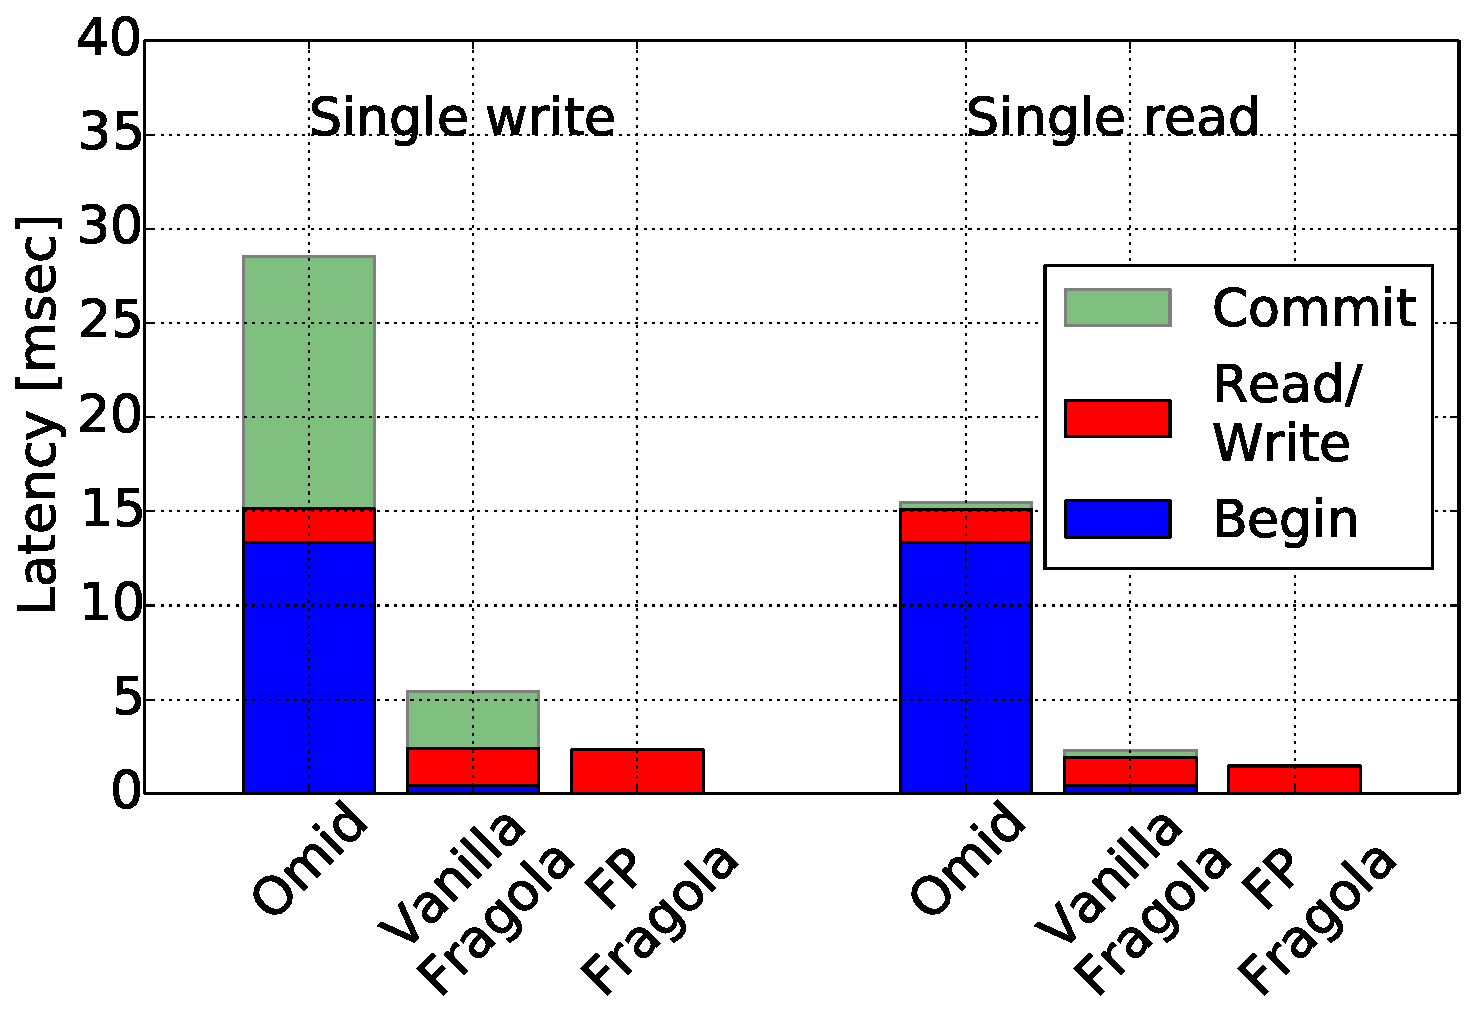
\includegraphics[width=\textwidth]{figs/latency_PUTGET.pdf}
        \caption[]{Single-key transaction latency breakdown at 100K tps.}
        \label{fig:stack-brc}
      \end{subfigure}  & 

\end{tabular}
       \caption{Latency vs.\ throughput and latency breakdown  for single-key transactions under  random mix workload. }
\end{figure*}

\paragraph{Results.} 

Recall that \sys\ is motivated by the prevalence of short transactions in production, and is designed with
the goal of speeding such transactions up.
Its advantage is less pronounced for long transactions, where the cost of begin and commit is amortized
across many reads and writes.
To make the comparison meaningful, we classify transactions according to their lengths and whether they
access a single key, and study each transaction class separately. 

We begin with short transactions. 
Figure~\ref{fig:tl-1} presents the average latency of single-key transactions run as part of the random mix,
as a function of {system} throughput.
Figure~\ref{fig:stack-brc}  then zooms in on the latency of such transactions under 
a throughput of 100K tps, and breaks up the different factors contributing to it. 

As we can see, under light load, \sys\ improves the latency of Omid by 4x to 5x, even without the fast path.
This is because in Omid, both begin and commit wait for preceding transactions to complete the writes of 
their commit entries; this stems from Omid's design choice to avoid the need for resolving pending write intents
by aborting transactions; see last (rightmost) column in Table~\ref{table:design-space}. 
Single-key writes suffer from both the begin and commit latencies, whereas single-key reads  
suffer only from begins (Figure~\ref{fig:stack-brc}). 

As load increases, \sys\ scales almost perfectly, whereas Omid suffers from a well-pronounced 
bottleneck. For instance, Omid's single-key transaction latency soars to 75ms under 300K tps whereas
{\sys}'s latency remains almost flat. The extra delay in Omid is due to batching of commit record updates, 
which its TM applies to handle congestion~\cite{Omid2017}. Such congestion arises due to Omid's centralized 
commit entry management (penultimate column in Table~\ref{table:design-space}).

The FP API delivers better performance for this traffic. For instance, single writes take an average of 2.4ms using 
the {\code bwc} API versus 5.4ms using the regular transaction API (consisting of begin, write, and commit). 
For comparison, a native HBase write takes roughly 2ms under this load.
A single read executed using {\code brc} takes 1.5ms, which is the average latency of a native HBase read,
versus 2.3ms as a regular transaction. 

\begin{figure}[htb]
\centering
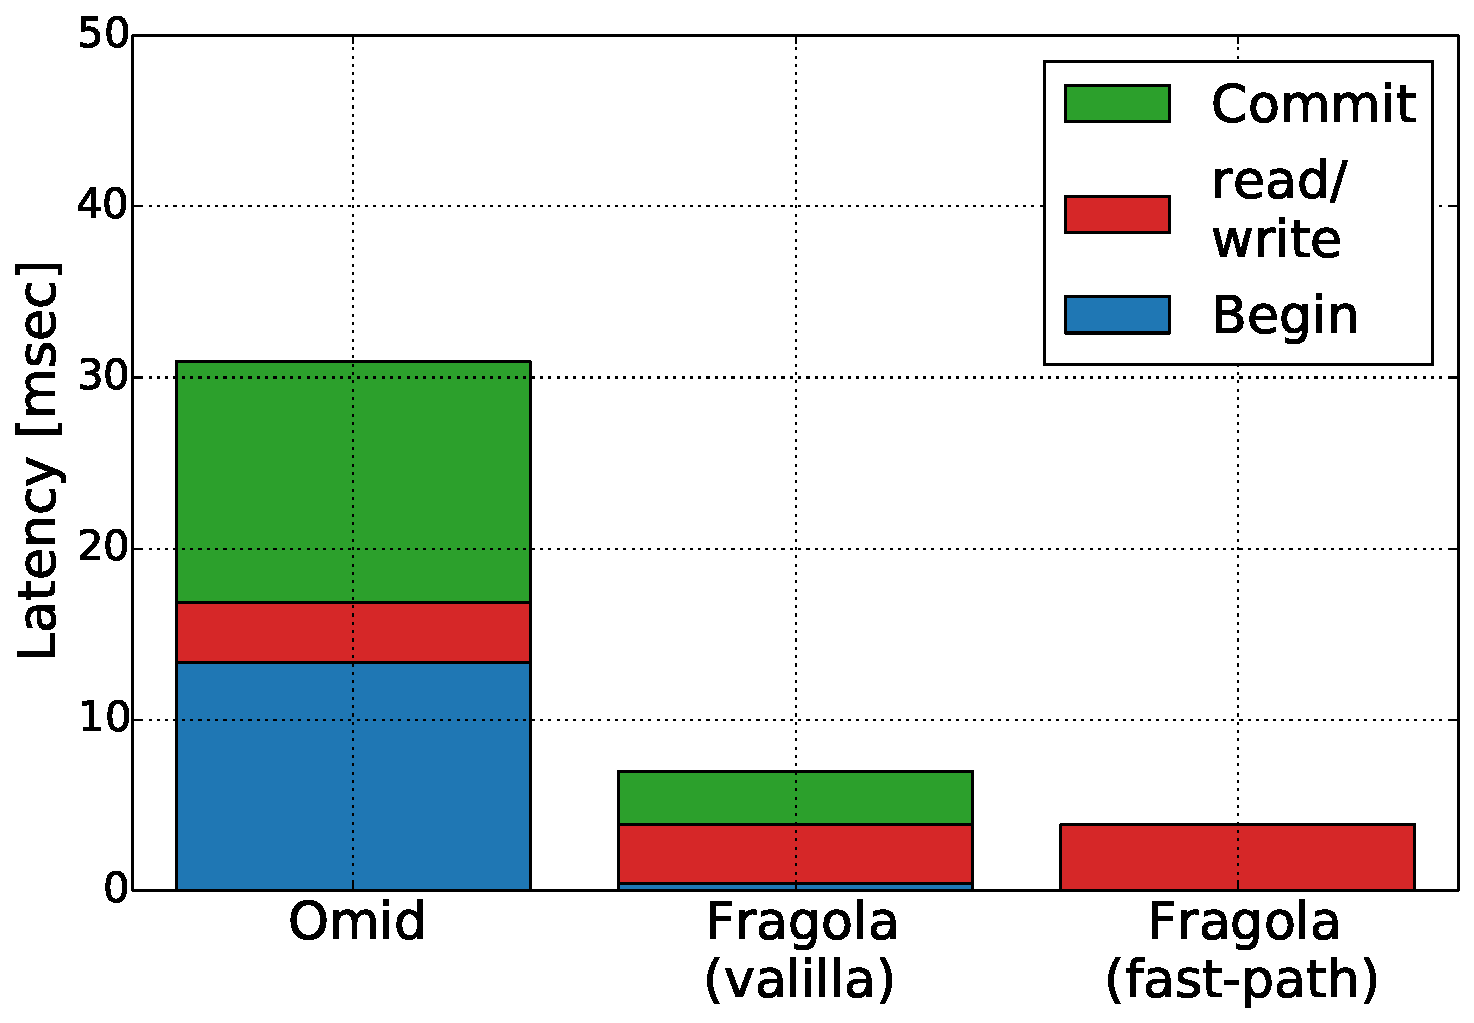
\includegraphics[width=.48\textwidth]{figs/latency_rwm.pdf}
\caption{Latency breakdown of single-key read+write transactions in the BRWC workload,
at 100K tps.}
\label{fig:rmw}
\end{figure}

We next focus on transactions that read and write a single key as part of the BRWC workload. 
Their latency breakdown under a 100K tps throughput is shown in Figure~\ref{fig:rmw}.
The fast path implementation (consisting of \code{br} and \code{wc} calls) completes within 3.9ms,
versus 7ms for Vanilla \sys\ and 30.9ms for Omid. 

We now examine longer transactions run as part of the random mix workload.
Figure~\ref{fig:throughput-latency} shows the results for transactions of lengths $5$ and $10$.
We see that the latency gap of \sys\ over Omid remains similar, but is amortized 
by other operations. Omid's control requests (begin and commit) continue to 
dominate the delay, and comprise $61\%$ of the latency of 10-access transactions.
In contrast, \sys's transaction latency is dominated by data access. For example, in 10-operation transactions only 
$17\%$ of the time is spent on the control path, which leads to much faster completion. 

\begin{figure*}[t]
\centering{
\begin{tabular}{cc}
\remove{
    \begin{subfigure}[t]{0.48\textwidth}
	\includegraphics[width=\textwidth]{figs/throughputlatency5.pdf}
	\caption[]{Throughput versus latency, transaction size = 5}
    \label{fig:tl-5}
  \end{subfigure} &
}
    \begin{subfigure}[t]{0.48\textwidth}
	\includegraphics[width=\textwidth]{figs/throughputlatency10.pdf}
	\caption[]{Throughput versus latency, transaction size = 10}
    \label{fig:tl-10}
  \end{subfigure} & 

\remove{
   \begin{subfigure}[t]{0.48\textwidth}
	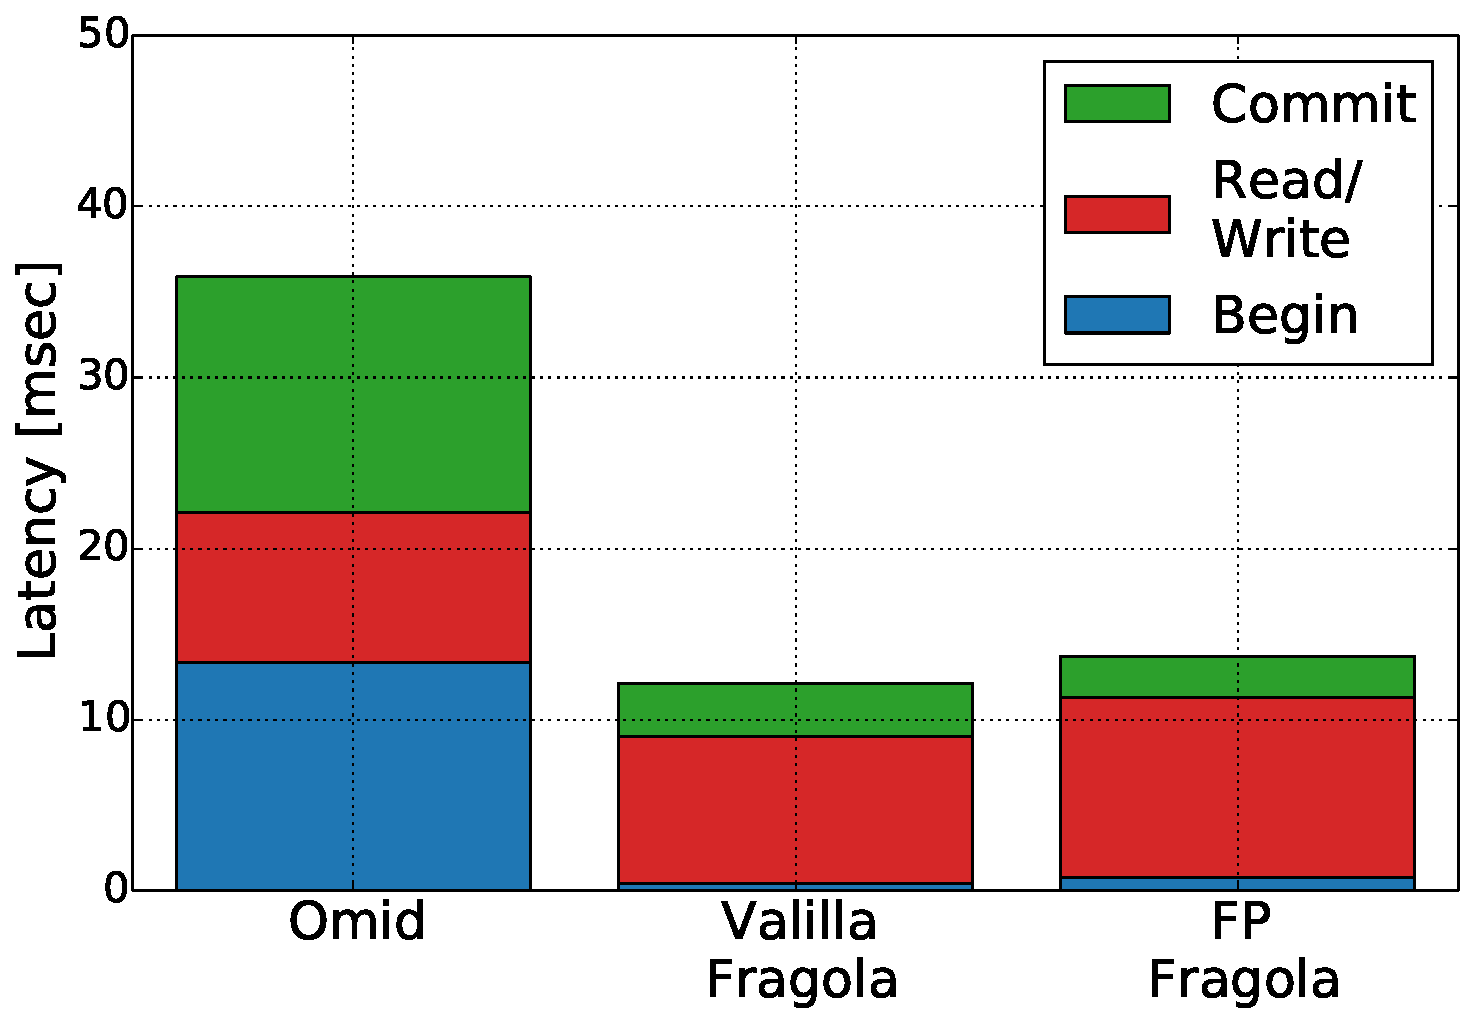
\includegraphics[width=\textwidth]{figs/latency_tx5.pdf}
	\caption[]{Latency breakdown, transaction size = 5}
    \label{fig:stack-tx5}
  \end{subfigure} &
  }
  \begin{subfigure}[t]{0.48\textwidth}
	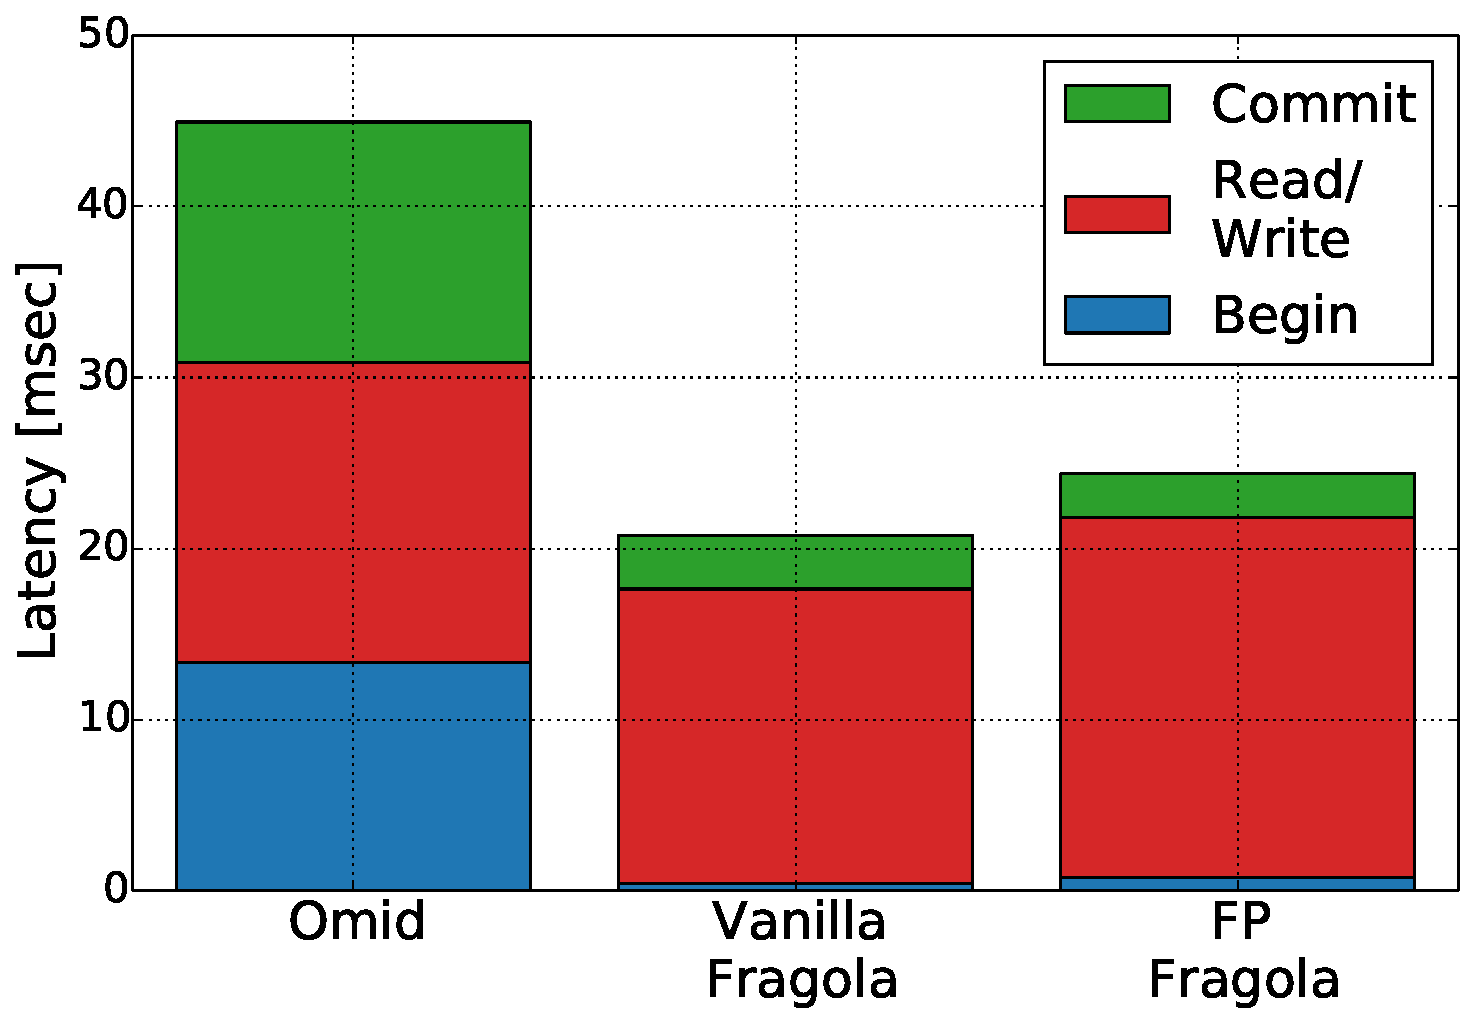
\includegraphics[width=\textwidth]{figs/latency_tx10.pdf}
	\caption[]{Latency breakdown, transaction size = 5, 10}
    \label{fig:stack-tx10}
  \end{subfigure} 
\end{tabular}  	
}		
  \caption{Latency vs.\ throughput  and latency breakdown  for long transactions in random mix workload. }
  \label{fig:throughput-latency}
\end{figure*}


Nevertheless,
the FP mechanism takes its toll on the data path, which resorts to atomic check\&mutate operations 
instead of simple writes. This is exacerbated for long transactions. 
For example, a 10-access transaction takes 24.4ms with FP \sys, 
versus 20.8ms with Vanilla \sys. 

\begin{figure}[h!]
\centering
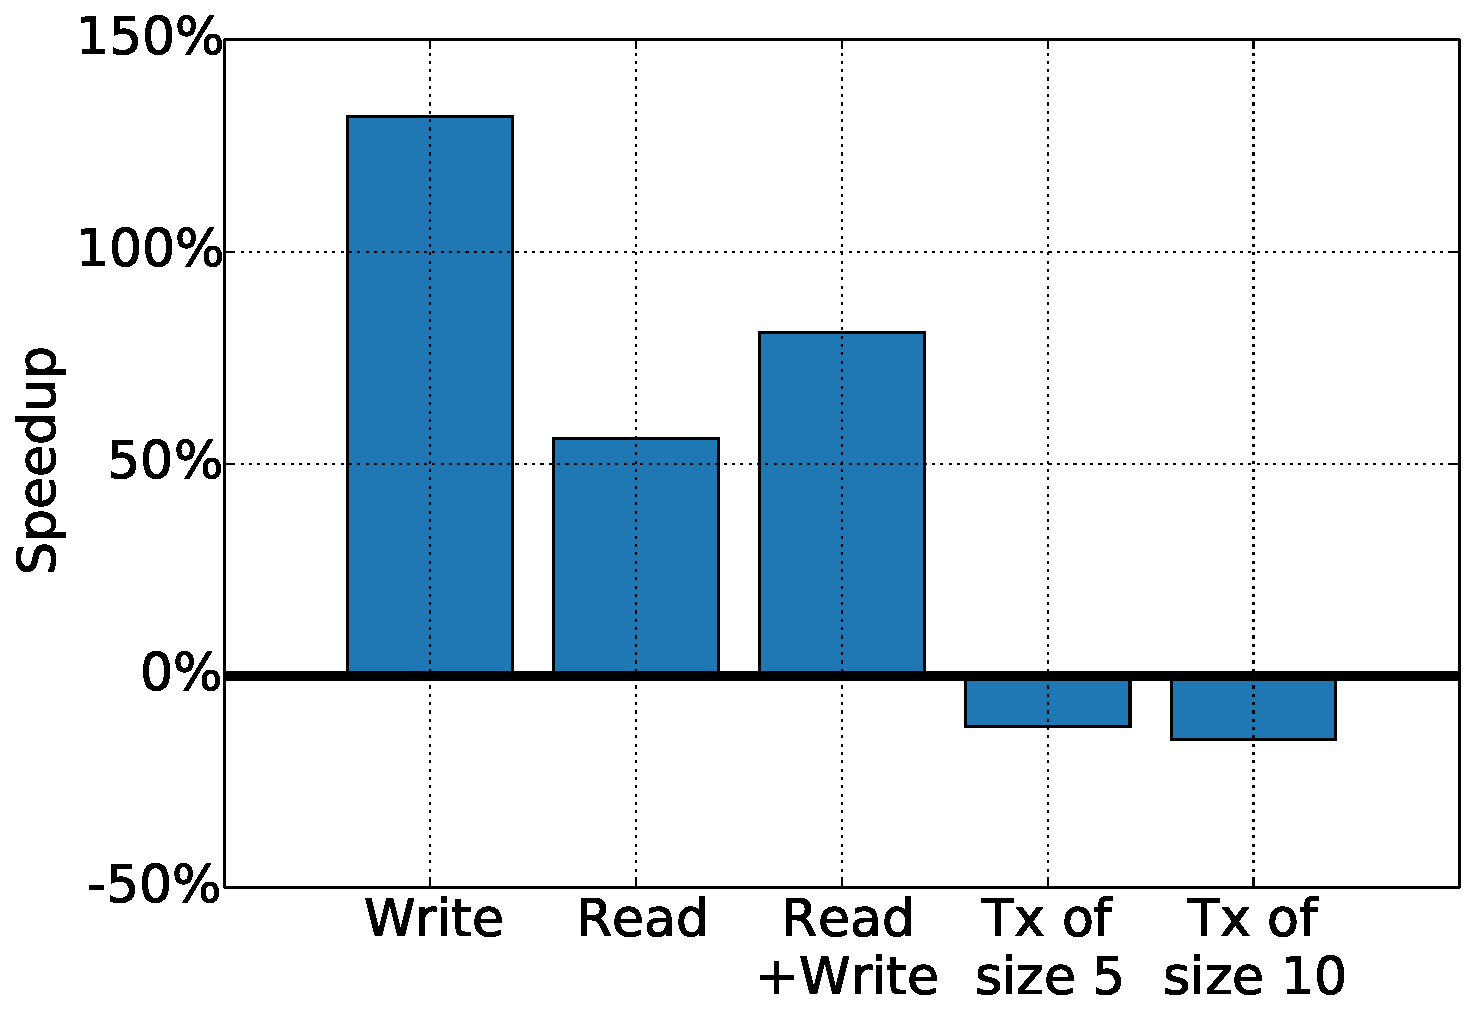
\includegraphics[width=.48\textwidth]{figs/speedup.pdf}
\caption{Summary of performance tradeoffs with the fast path API in {\sys}.}
\label{fig:fp-tradeoff}
\end{figure}

Figure~\ref{fig:fp-tradeoff} summarizes the performance tradeoffs entailed by the fast path API
(relative to Vanilla Fragola) for the different transaction classes. 
We see that the speedup for single-write transactions is 2.3x, whereas the worst slowdown is $14.8\%$. 
In systems geared towards real-time processing, this is a reasonable tradeoff, since long transactions 
are infrequent and less sensitive to extra delay. Under the studied workload, e.g.,   FP \sys\/ is more desirable. 

We note that \sys\/ yields slightly higher rates of transaction aborts compared to Omid (recall 
that Vanilla \sys\/ aborts tentative writes in favor of concurrent reads, whereas FP \sys\/ also aborts
singleton writes in presence of concurrent tentative writes). However, the abort rates exhibited by all  
the systems are minor. Here, under the highest contention, FP \sys\/ aborts approximately $0.1\%$ 
of the transactions vs Vanilla \sys's $0.08\%$ and Omid's $0.07\%$ (the latter  is in line 
with~\cite{Omid2017}).  



\Idit{Compare the following: Omid 2, regular transactions in \sys, local transactions in \sys, HBase.}

\Idit{Add graph showing cost of RMW (validation) in regular transaction write.}

\section{Related Work} \label{sec:related}

\section{Conclusion} \label{sec:conclusions}



%\subsection*{Acknowledgments}

\newpage

\bibliographystyle{acm}
\bibliography{main}


%%%%%%%%%%%%%%%%%%%%%%%%%%%%%%%%%%%%%%%%%%%%%%%%%%%%%%%%%%%%%%%%%%%%%%%%%%%%%%%%%%%%%%%%%%%%%%%%%%%%%%%%%%%%%%%%%%%%%%%%%%%%%%%%%%%%
% Appendix
%%%%%%%%%%%%%%%%%%%%%%%%%%%%%%%%%%%%%%%%%%%%%%%%%%%%%%%%%%%%%%%%%%%%%%%%%%%%%%%%%%%%%%%%%%%%%%%%%%%%%%%%%%%%%%%%%%%%%%%%%%%%%%%%%%%%

%\newpage

\begin{appendix}
	
	\section{Notations and definitions} \label{sec:app1}


\end{appendix}
%%%%%%%%%%%%%%%%%%%%%%%%%%%%%%%%%%%%%%%%%%%%%%%%%%%%%%%%%%%%%%%%%%%%%%%%%%%%%%%%%%%%%%%%%%%%%%%%%%%%%%%%%%%%%%%%%%%%%%%%%%%%%%%%%%%%


\end{document}
